\RequirePackage{luatex85}\documentclass[beamer,xcolor={table,rgb,dvipsnames}]{beamer}
%*****************************************************************************
%** beamer setup  **************************************************************

\usecolortheme{rose}
%\usetheme[wide]{sra}
\usetheme[wide,bgstyle=osg]{sra}

\setbeamertemplate{navigation symbols}{}

\usepackage[sracolors,autonotes]{beamertools}

\usepackage{csquotes}
\usepackage{booktabs}
\usepackage{xspace}
\usepackage{multirow}
\usepackage{pgffor}

\usepackage{iftex}
\ifluatex
  \usepackage{lmodern}
  \usepackage[no-math]{fontspec}
  % VeraMono ist viel schmaller als Beramono
  \setmonofont{VeraMono}[
     Extension       = .ttf,
     BoldFont        = *-Bold,
     ItalicFont      = *-Italic,
     BoldItalicFont  = *-Bold-Italic,
     Scale           = MatchLowercase,
  ]
  \usepackage{pifont}
\else
  \usepackage[utf8]{inputenc}
  \usepackage[T1]{fontenc}
  \usepackage{helvet}
  \usepackage{pifont}
  \usepackage[scaled=0.85]{beramono}
\fi

\long\def\maketitleframe{
  \begin{frame}
    \maketitle
  \end{frame}
}


\newcommand{\dividerframe}[1]{
  \begin{frame}
    \begin{center}
      \Huge #1
    \end{center}
  \end{frame}
}

\AtBeginDocument{
  \pagenumbering{arabic} % for pageslts
}

% Customize numbering:
% We want to number frames as <chapter>-<frame> with <frame> being by-chapter numbers
% Note: The following works only if a patch is applied to beamerbaseframe.sty (see README)
\renewcommand{\theframenumber}{\arabic{framenumber}}
\renewcommand{\insertframenumber}{\theframenumber}
\renewcommand{\InsertFrameNumber}{\insertframenumber}

  \newcommand{\columntitle}[1]{
    {\centering\structure{\strut #1}\par}
  }


  \newcommand{\animation}[3][]{%
  \foreach \p/\s in {#2} {%
    \includegraphics<\s|handout:\s|skript:\s>[page=\p,#1]{#3}%
  }%
}

\usepackage{mdframed}


%*****************************************************************************
%** bibliography
%*************************************************************
\usepackage{polyglossia}
\setdefaultlanguage{german}

\usepackage[style=numeric-comp,hyperref,maxnames=3,minnames=3,defernums=true]{biblatex}
\defbibheading{bibliography}{}
\bibliography{bib/sra-own.bib}
\renewcommand{\bibfont}{\scriptsize}
\DeclareFieldFormat{postnote}{#1}



%****************************************************************
%** tikz stuff
\usepackage{tikz}
\usetikzlibrary{tikzmark,arrows,fit,calc,positioning,sra,shapes.multipart}
\usepackage{pgfkeys}
\tikzset{
  >=latex',
  small tree/.style={
    every node/.append style={
      font=\footnotesize,
      draw,
    },
    level distance=1cm,
  }
}

%*****************************************************************************
%** Legalcode *************************************************************

\pgfkeys{
  /legalcode/commons/.style={url={https://commons.wikimedia.org/wiki/File:#1}},
  /legalcode/url/.code={%
    \def\lcText##1{\href{#1}{##1}}
  },
  /legalcode/author/.code={\def\lcAuthor{, #1}},
  /legalcode/license/CC BY-SA 3.0/.code={%
    \def\lcLicense{\href{https://creativecommons.org/licenses/by-sa/3.0/legalcode}{CC BY-SA 3.0}}%
  },
  /legalcode/license/Free Art License/.code={%
    \def\lcLicense{Free Art License}%
  }
}
\newcommand{\legalcode}[3][]{% [opts]{license}{title}
  \bgroup%
  \def\lcText##1{##1}
  \def\lcAuthor{}
  \pgfkeys{/legalcode/.cd,#1,license/#2}%
  \parbox{\textwidth}{\centering\color{gray}\tiny\lcText{#3}\lcAuthor{} \mbox{(\lcLicense)}}
  \egroup
}

\colorlet{codecolor}{luhlightgray!50}
\usepackage{lecturesourcecode}




%*****************************************************************************
%** code blocks **************************************************************

  \makeatletter
  \setbeamercolor{code}{fg=black,bg=codecolor}

  \define@key{beamercolbox}{text width}{\pgfmathsetlengthmacro{\beamer@colbox@wd}{#1}}
  \define@key{beamercolbox}{text height}{\pgfmathsetlengthmacro{\beamer@colbox@ht}{#1}}
  \define@key{beamercolbox}{text depth}{\pgfmathsetlengthmacro{\beamer@colbox@dp}{#1}}
  \define@key{beamercolbox}{background color}{\setbeamercolor{code}{fg=black,bg=#1}}
  \define@key{beamercolbox}{scale content}{\def\bt@innerscale{#1}}
  \define@key{beamercolbox}{tag}{\def\bt@tag{#1}}

  \newenvironment<>{code}[1][\empty]{%
    \begin{onlyenv}#2%
    \vspace{2pt}%
    \setkeys{beamercolbox}{#1}
    \lstset{aboveskip=0pt,belowskip=0pt,linewidth=\beamer@colbox@wd}%
    \rule{2pt}{0pt}\begin{beamercolorbox}[colsep*=2pt,text width=\linewidth-4pt, text depth=0ex,#1]{code}%
    \ifdef\bt@innerscale{%
      \pgfmathsetlength{\@tempdima}{\beamer@colbox@wd/\bt@innerscale}
      \begin{adjustbox}{scale=\bt@innerscale}
      \begin{minipage}{\@tempdima}
        \lstset{linewidth=\@tempdima}%
      }{}
  }{%
    \ifcsdef{bt@tag}{%
      \vspace{-1.2\baselineskip}\hfill{\emph{\color{black!70!white}\csuse{bt@tag}}}
      \vspace{0.4\baselineskip}
    }{}%
    \ifdef\bt@innerscale{%
      \end{minipage}
      \end{adjustbox}
    }{}%
    \end{beamercolorbox}\rule{2pt}{0pt}\vspace{2pt}%
    \end{onlyenv}%
    \ignorespacesafterend%
  }

  \usepackage{xparse}
  \usepackage{realboxes}


%%%%%%%%%%%%%%%%%%%%%%%%%%%%%%%%%%%%%%%%%%%%%%%%%%%%%%%%%%%%%%%%
% Misc

\setbeamercolor{advantage text}{fg=safegreen!80!black}
\newenvironment{advantageenv}{\begin{altenv}%
    {\usebeamertemplate{advantage text begin}%
      \usebeamercolor[fg]{advantage text}%
     \usebeamerfont{advantage text}}
    {\usebeamertemplate{advantage text end}}{\color{.}}{}}{\end{altenv}}

\newcommand<>{\advantage}[1]{\hskip0pt\begin{advantageenv}#2#1\end{advantageenv}}
\newcommand<>{\Advantage}[1]{\advantage#2{\emph#2{#1}}}
\newcommand<>{\ADVANTAGE}[1]{\advantage#2{\textbf#2{#1}}}

\newcommand{\dn}[2][]{\tikz[baseline]\node[anchor=base,circle,inner sep=1pt,draw,every dn/.try,#1]{#2};}
\renewcommand{\iiad}{\ii[\color{safegreen}\textbf{+}]}  % advantage
\renewcommand{\iida}{\ii[\color{safered}\textbf{--}]} % disadvantage
\newcommand{\lecturetag}[3][]{%
  \tikz[baseline]\node[anchor=base,draw=black,fill=#2color,#1]{\color{black}Vorlesung #3};
}

\newcommand{\tikznode}[2][]{%
  \tikz[baseline,remember picture]\node[anchor=base,#1]{#2};%
}
\newenvironment<>{tikznodeenv}[1][]{%
  \begingroup%
  \tikzset{tikznode@style/.style={#1}}%
  \begin{lrbox}{\@tempboxa}%
}{\end{lrbox}%
  \tikz[remember picture]\node[inner sep=0,outer sep=0, tikznode@style]{\usebox{\@tempboxa}};
  \endgroup%
}

\newenvironment<>{visible}[1][]{\begin{scope}[visible on=#2,#1]}{\end{scope}}

\newsavebox{\@overlaybox}
\def\@overlayboxType{\vbox}
\def\overlayboxHBOX{\let\@overlayboxType=\hbox}
\newenvironment<>{overlaybox}[1][]{%
  % We set the overlay tikz node in the next shipout routine.
  % Thereby, we do not produce a \leavemode after the lrbox
  \only#2{%
    \AtBeginShipoutNext{%
      \AtBeginShipoutUpperLeftForeground{%
        \begin{tikzpicture}[remember picture, overlay]%
          \node[fill=white,draw] at (current page.center) [#1] {\usebox{\@overlaybox}};
        \end{tikzpicture}%
      }%
    }%
  }%
  % Produce the @conclusionoverlay
  \setbox\@overlaybox=\@overlayboxType\bgroup%
}{%
  \egroup%
  \global\setbox\@overlaybox=\copy\@overlaybox\relax%
}

%\usepackage{default}
\makeatletter
\newif\ifOnBeamerModeTransition
\newcommand{\slideselection}{1-}%
\newenvironment{handoutframeselect}[1][1-]{%
  \begingroup%
  \mode<handout>{%
    \gdef\beamer@currentmode{beamer}%
    \OnBeamerModeTransitiontrue%
    \renewcommand{\slideselection}{#1}}%
}{%
  \ifOnBeamerModeTransition%
    \OnBeamerModeTransitionfalse%
    \gdef\beamer@currentmode{handout}%
  \fi%
  \endgroup%
}
\makeatother


\makeatletter
\newsavebox{\@btModalBox}
\newenvironment<>{btModal}[1][]{%
  \begingroup%
  \gdef\@btModalStyle{fill=white,#1}%
  \def\@btModalOverlay{#2}% <overlayspec>
  \begin{lrbox}{\@btModalBox}%
  }{%
  \end{lrbox}%
  \global\setbox\@btModalBox=\copy\@btModalBox\relax%
  \expandafter\only\@btModalOverlay{%
    \AtBeginShipoutNext{%
      \AtBeginShipoutUpperLeftForeground{%
        \begin{tikzpicture}[remember picture, overlay]%
          \node[opacity=0.4,anchor=center,at=(current page.center),anchor=center,fill=luhgray,minimum width=\paperwidth,minimum height=\paperheight]{};
          \expandafter\node\expandafter[\@btModalStyle] at (current page.center) {\usebox{\@btModalBox}};
        \end{tikzpicture}%
      }%
    }%
  }%
  \endgroup%
}
\makeatother


\def\TAG#1{\hfill\raisebox{0.5\baselineskip}{\emph{#1}}}

  \newcommand{\InsertBibliography}{
    % if in \master mode, bib-items will be collected at the very end
    \ifx\master\undefined
      \subsection{Referenzen}
      \begin{frame}[allowframebreaks]
        \frametitle{Referenzen}
        \printbibliography
      \end{frame}
    \fi
  }

\usepackage{pageslts} %  theCurrentPage
\usepackage{calc} % theCurrentPage


\author{Christian Dietrich}
\date{13. September 2021}
\AtBeginDocument{
  \pagenumbering{arabic} % for pageslts

  \btset{
        pdfframes/.cd,
        clear/accent color={tuhhcyan},
        clear/logo insert={%
          \rlap{%
            \raisebox{\dimexpr\paperheight-4.219pt-16.765pt\relax}{%
              \rule{7.139pt}{0pt}\includegraphics[width=16.765pt]{tuhh-osg-logo}%
            }%
          }%
        },
      }
}


\begin{document}

\subtitle{Between Static Configuration and Dynamic Reconfiguration}
\title{Semi-Dynamic Variability}


\begin{frame}[title]
  \maketitle
\end{frame}

\begin{frame}<0>[label=toc]{Agenda}

  \alt<2,4>{
    \colorlet{mvBG}{safegreen!15}
  }{
    \colorlet{mvBG}{white}
  }
\begin{mdframed}[linecolor=safegreen!40,backgroundcolor=mvBG ,
                 linewidth=5pt,topline=false,rightline=false,bottomline=false,  innertopmargin=6pt, innerbottommargin=6pt, innerleftmargin=6pt, innerrightmargin=6pt]


  \begin{minipage}{0.1\linewidth}
    
\includegraphics[width=\linewidth]{fig/multiverse.png}
  \end{minipage}\hfill%
  \begin{minipage}{0.87\linewidth}
  {\LARGE Multiverse}\alt<-3>{\TAG{EuroSys'19}}{}\\
  {\large Efficient Semi-Dynamic Variability}
\end{minipage}\\[1.5ex]

  \bii
  \ii Preparing variants at compile time
  \ii Efficient binding by run-time code patching
  \eii
\end{mdframed}\vspace{1cm}

  \alt<3,4>{
    \colorlet{wfBG}{luhblue!15}
  }{
    \colorlet{wfBG}{white}
  }
\begin{mdframed}[linecolor=luhblue!40,backgroundcolor=wfBG,linewidth=5pt,topline=false,rightline=false,bottomline=false,  innertopmargin=6pt, innerbottommargin=6pt, innerleftmargin=6pt, innerrightmargin=6pt]


  \begin{minipage}{0.1\linewidth}
    
\includegraphics[width=\linewidth]{fig/wfpatch.pdf}
  \end{minipage}\hfill%
  \begin{minipage}{0.87\linewidth}
  {\LARGE Wait-free code patching}\alt<-3>{\TAG{OSDI'20}}{}\\
  {\large Run-time code patching without interruption}
\end{minipage}\\[1.5ex]

  \bii
  \ii Preparing changes in a separate address space
  \ii Incremental migration of threads
  \eii
\end{mdframed}  

\end{frame}
% \OrgLectureSectionStop{}{19-74}

% \qq{Variabilität}{76-109}
%  \begin{frame}[t]{Adaptive Systemsoftware}
%    \btAnimation[width=0.9\linewidth]{center,padding=2ex,range=1-8:<1->,8:<9->}{fig/02-requirements}
%
%    \begin{columns}[t]
%      \begin{column}{0.4\textwidth}
%        \structure{Beispiel: Linux}
%        \bii
%        \ii $>30$ \hspace{3mm}\btSetTab Architekturen
%        \ii $>15$k \btUseTab Features
%        \ii $>27$m \btUseTab Lines of Code
%        \ii<2-> Komplexes Featuremodell
%        \ii<7-> $>80$k \btUseTab Commits/Jahr
%        \eii
%      \end{column}\hfill
%      \begin{column}<2->{0.55\textwidth}
%        \structure{Verwender: Ich habe Wünsche!}
%        \bii
%        \ii<2-> Passend zum Anwendungsprofile
%        \ii<5-> Fehlerbehebung durch Introspection
%        \ii<6-> Anpassbarkeit vor/während der Laufzeit
%        \ii<7-> Erweiterbar um Spezialfeatures
%        \ii<8-> Updates ohne Unterbrechungen
%        \eii
%      \end{column}
%    \end{columns}
%    \vspace{2ex}
%
%    \uncover<9>{\OrangeBox{\emph{Ein variables System kann sich den Wünschen des Verwender anpassen.}}}
%  \end{frame}
%  
% \OrgLectureSectionStop{Variabilität}{76-109}

% \OrgLectureSectionStart{Variabilität}{109-119}
\btInputPDFFrames{%
  file=fig/motivational-en,
  clear={not title},
  title={},
  single frame,
  range={1,...,7}
}
% \OrgLectureSectionStop{Variabilität}{109-119}

% \OrgLectureSectionStart{Variabilität}{119-194}
\begin{frame}[t,fragile]{Static and Dynamic Variability}
\structure{Creation}: \btSetTab of a variant's binary form\\
\structure{Binding}:  \btUseTab Integration of Variant into Program\\

  \bigskip
  \begin{columns}[b]
    \begin{column}<2->{0.49\textwidth}
      \begin{code}[]
        \begin{C}
          #ifdef CONFIG_SMP
          irq_disable();
          spin_acquire(&lock);
          #else
          irq_disable();
          #endif
        \end{C}
      \end{code}
    \end{column}\hfill
    \begin{column}<3->{0.49\textwidth}
      \begin{code}<0>[]
        \begin{C}
          if (config_smp) {
            fn  = dlsym("smp.so", "acquire");
            fn(&lock);
          } else {
            irq_disable();
          }
        \end{C}
      \end{code}%
      \begin{code}<3->[]
        \begin{C}
          if (config_smp) {
            irq_disable();
            spin_acquire(&lock);
          } else {
            irq_disable();
          }
        \end{C}
      \end{code}
    \end{column}
  \end{columns}

  \begin{columns}[t]
    \begin{column}<2->{0.49\textwidth}
      \columntitle{Static Variability}
      \bii
      \ii Creating: \btSetTab Compile-Time
      \ii Binding:        \btUseTab Compile-Time\\[1ex]
      \iiad No Run-Time Overhead
      \iida Each combination: A different binary
      \eii


    \end{column}\hfill
    \begin{column}<3->{0.49\textwidth}
      \columntitle{Dynamic Variability}
      \bii
      \ii Creation: \btSetTab Hybrid Variants\\
      \ii Binding: \btUseTab Time-of-Use\\[1ex]
      \iida Repeated binding costs
      \iiad Flexible and reconfigurable
      \eii
    \end{column}
  \end{columns}
  \medskip
  \begin{btBlock}<4>{$\leadsto$ Semi-Dynamic Variability}\small
    Static Creation and \textbf{efficient} dynamic (re-)binding
  \end{btBlock}



\end{frame}

% \OrgLectureSectionStop{Variabilität}{119-194}

% \OrgLectureSectionStart{Multiverse}{195-249}
\againframe<1-2>{toc}


\makeatletter
\bt@pdfframes@onpagehook
\makeatother

\btInputPDFFrames{%
  file=talks/multiverse.pdf,
  clear,
  title={Creation: Compiler Plugin},
  single frame,
  range={30,...,33}
}

\btInputPDFFrames{%
  file=talks/multiverse.pdf,
  clear,
  title={Bindung: Run-Time Code Patching},
  single frame,
  range={34,35,36,37,40}
}


\btInputPDFFrames{%
  file=talks/multiverse.pdf,
  clear,
  title={Semi-Dynamic Locks in Kernel/Userspace},
  single frame,
  range={41,42,43},
  on page={43}{%
    add content={
      \begin{btModal}<2-> [draw=safegreen,ultra thick,inner sep=2ex,name=modal,
        tikz content={
          \draw[line width=2ex,safegreen] (modal.north west) -- (modal.south west);
        },
        ]
        \begin{minipage}{0.8\linewidth}
          \structure{Multiverse -- Efficient Semi-Dynamic Variability}
          \bii
          \iiad Variability specification within language
          \iiad Run-time cost like static variability
          \iiad Flexibility like dynamic variability\\[2ex]
          \iida<3-> Binary file increases in size
          \iida<3-> Run-time code patching requires synchronization
          \eii
        \end{minipage}
      \end{btModal}
    }
  },
}

\IfFileExists{secret-slides.tex}{
  \begin{frame}{Tutorial: Virtual Machine and SSH Host}
  \bi
  \ii Example Source Code {
    \bi
    \ii \texttt{git clone https://github.com/luhsra/multiverse-atlas-demo.git}
    \ii \texttt{./init} => Clone dependent Libraries
    \ii You need a mmview-enabled kernel for example 02/03
    \ei
  }
  \ii Virtual Machine Image {
    \bi
    \ii Download: \url{FIXME}
    \ii Start: \texttt{qemu-system-x86\_64 -m 4G -enable-kvm -hda hda.qcow2 -smp 4}
    \ii User/Passwort: \texttt{root/root}, \texttt{user/user}
    \ei
  }
  \qquad
  \ii Running Virtual Machine (temporary) {
    \bi
    \ii \texttt{ssh user@lab.sra.uni-hannover.de -p 2250}
    \ii Password: \texttt{FIXME}
    \ii Machine will be available only for the time of the tutorial.
    \ei
  }
  \ei
  
\end{frame}

}{}


\begin{frame}[fragile]{Tutorial: 01-multiverse}
  \begin{btBlock}{Goal}
    Demonstrate Semi-Dynamic Lock-Elision with Multiverse
  \end{btBlock}

  \bi
  \ii Static Creation with \texttt{\_\_attribute\_\_((multiverse))}{
    \bi
    \ii Multiverse Variables (MV) are \enquote{features}. Default Range: \{0, 1\}
    \ii Attributed functions are multiversed at MV usages.
    \ii Cross-Product of MV ranges.
    \ei
  }
  \ii Binary File: \texttt{01-multiverse} {
    \bi
    \ii Regular functions: \texttt{lock()}, \texttt{unlock()}
    \ii Use \texttt{objdump -d 01-multiverse} to inspect assembler
    \ii Search for \texttt{lock.multiverse.smp\_0}
    \ei
  }
  \ii Multiverse Metadata
  \begin{code}
    \begin{codetext}
  fn: lock 0x55bd78dc92e0, 2 variants
    mvfn: 0x55bd78dc9410 (vars 1)
      assign: smp in [0, 0]
    mvfn: 0x55bd78dc9420 (vars 1)
      assign: smp in [1, 1]
    \end{codetext}
  \end{code}
  \ei
\end{frame}


\begin{frame}[fragile,t]{Tutorial: 01-multiverse}
  \framesubtitle{Backup Results}
  \begin{columns}
    \begin{column}{0.49\textwidth}
      \begin{code}[]
        \begin{codetext}
Without Multiverse (smp=0)
 work() -> 83.376870 ms
 work() -> 70.550493 ms
 work() -> 70.670475 ms
 work() -> 70.578593 ms
 work() -> 73.273835 ms
Average (n=5): 73.690053

Without Multiverse (smp=1)
 work() -> 511.101093 ms
 work() -> 511.533894 ms
 work() -> 512.103367 ms
 work() -> 519.490820 ms
 work() -> 511.268393 ms
Average (n=5): 513.099513
        \end{codetext}
      \end{code}
    \end{column}\hfill
    \begin{column}{0.49\textwidth}
\begin{code}[]
  \begin{codetext}
With Multiverse (smp=0)
 work() -> 18.856244 ms
 work() -> 18.820774 ms
 work() -> 18.878794 ms
 work() -> 18.757183 ms
 work() -> 18.795324 ms
Average (n=5): 18.821664


With Multiverse (smp=1)
 work() -> 509.799176 ms
 work() -> 509.639876 ms
 work() -> 518.221404 ms
 work() -> 511.009342 ms
 work() -> 510.144087 ms
Average (n=5): 511.762777
  \end{codetext}
\end{code}
    \end{column}
  \end{columns}

  
\end{frame}

\againframe<3>{toc}

\begin{frame}{Global Quiescence}
  \begin{center}
    \OrangeBox{Run-Time Code Patching requires Quiescence!}
    \bigskip

    \btAnimation[width=0.7\linewidth]{range=1-4:<1->,5:<5->}{fig/02-timeline.pdf}

    \bigskip
    \bi
    \iida<3-> Global barrier bears risk of dead-lock
    \iida<3-> Impact on service quality
    \iiad<4-> Strong consistency through global quiescence
    \ei
  \end{center}
  \begin{btModal}<6>[draw=srared,thick,inner sep=1em]
    \begin{minipage}{0.8\linewidth}
      \begin{center}
        {\Large\structure{OpenLDAP}} \\[2ex]

      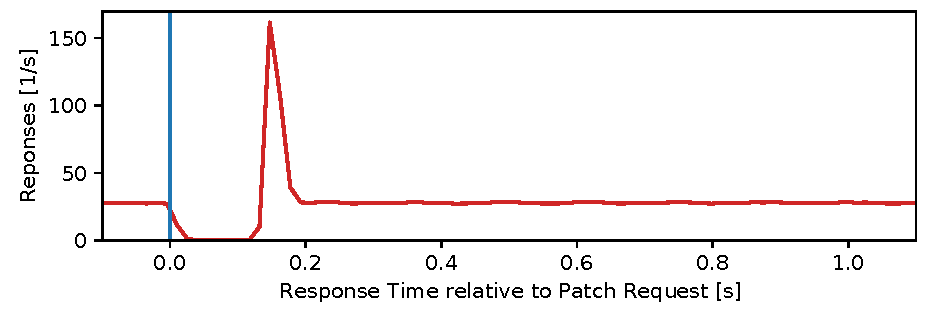
\includegraphics[width=0.6\pagewidth]{fig/request-1}\\[1ex]
      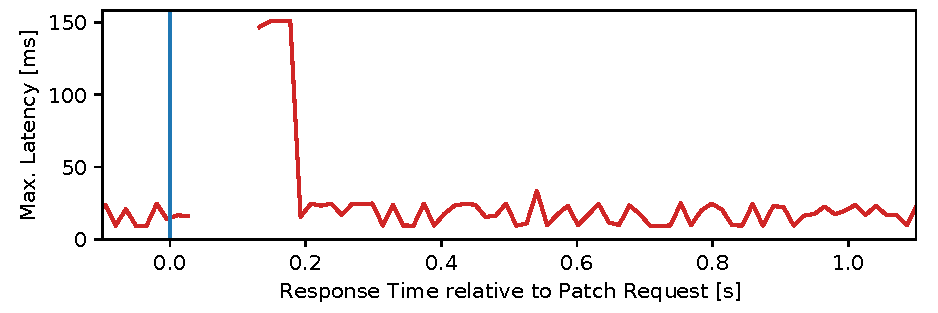
\includegraphics[width=0.6\pagewidth]{fig/request-2}
    \end{center}
    \end{minipage}
  \end{btModal}
\end{frame}


\begin{frame}{Global Quiescence $\rightarrow$ Local Quiescence}
  \begin{center}
    \btAnimation[width=0.7\linewidth]{1:<1->}{fig/02-local-quiescence.pdf}
  \end{center}


  \begin{btBlock}{Wait-Free Code Patching \hfill \emph{Incremental Application of Patch}}
    \bi
    \ii Prepare the modified code segment
    \ii Threads migrate themselves and without synchronization
    \ii Old and new variants co-exist (for shorter or longer periods of time)
    \ei
  \end{btBlock}


\end{frame}


\btInputPDFFrames{%
  file=talks/wfpatch.pdf,
  clear,
  title={Address-Space Views},
  single frame,
  range={29,...,38},
  on page={38}{%
    add content={
      \begin{btModal}<2-4>[draw=srared,thick,inner sep=1em]
        \begin{minipage}{0.8\linewidth}
          \begin{center}
            {\Large\structure{OpenLDAP}} \\[2ex]

            \alt<2>  {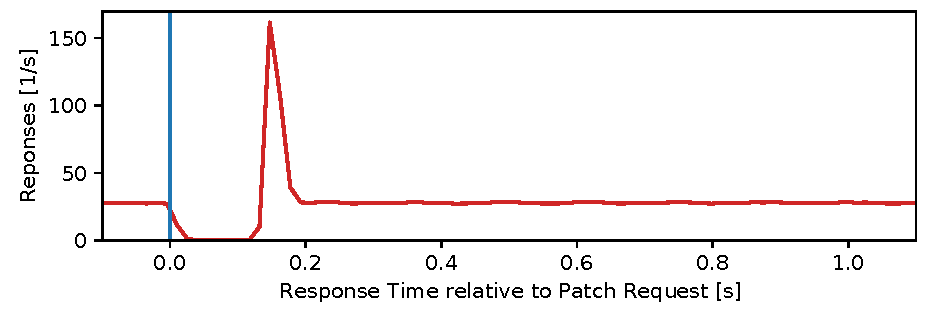
\includegraphics[width=0.6\pagewidth]{fig/request-1}}
                     {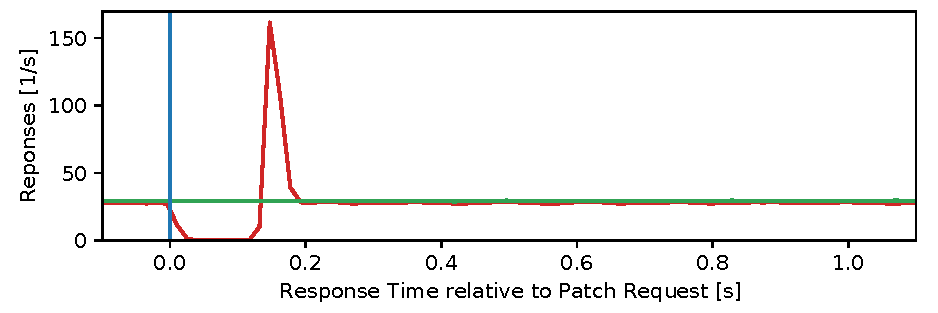
\includegraphics[width=0.6\pagewidth]{fig/request-3}}\\[1ex]
            \alt<2-3>{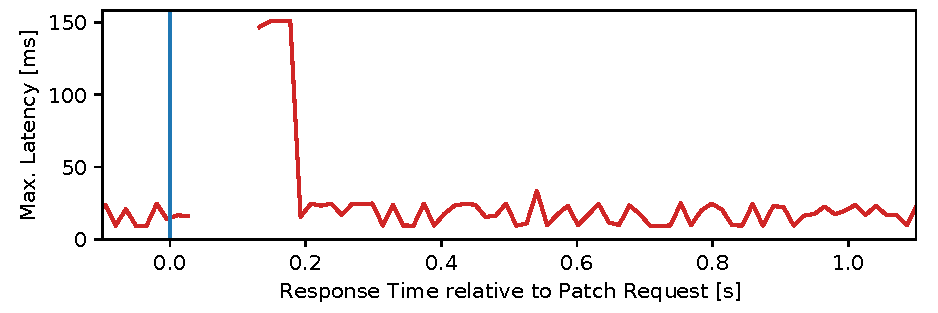
\includegraphics[width=0.6\pagewidth]{fig/request-2}}
                     {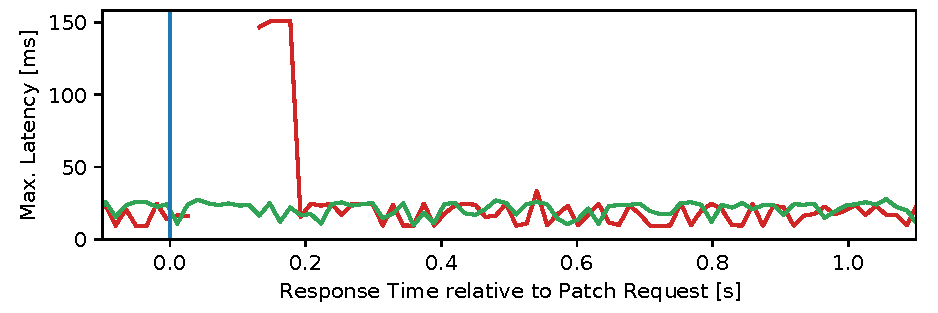
\includegraphics[width=0.6\pagewidth]{fig/request-4}}
          \end{center}
        \end{minipage}
      \end{btModal}
    }
  }
}

% \OrgLectureSectionStop{Wait-Free Code Patching}{251-359}
  \btInputPDFFrames{%
    file=talks/wfpatch.pdf,
    clear,
    title={Response Time Latencies},
    single frame,
    range={38},
    add content={%
      \begin{btModal}<1->[draw=luhblue,ultra thick,inner sep=1.5ex,name=modal,
        tikz content={
          \draw[line width=2ex,luhblue] (modal.north west) -- (modal.south west);
        },
        ]
        \begin{minipage}{0.8\linewidth}
          \begin{columns}
            \begin{column}{0.15\textwidth}
              
\includegraphics[width=\linewidth]{fig/server.png}
            \end{column}\hfill
            \begin{column}[c]{0.8\textwidth}
              \structure{Wait-Free Code Patching}
              \bii
              \iiad Service quality and progress remain steady
              \iiad No problem with deadlocks
              \iida Weaker consistency guarantees\\[1ex]
              \ii \textbf{Different Applications:}\\Multiverse, Dynamic Updates, JIT, Tracing
              \eii
            \end{column}
          \end{columns}
        \end{minipage}
        \end{btModal}
     }
  }


  \begin{frame}[fragile]{Tutorial: 02-migrate}
  \begin{btBlock}{Goal}
    Demonstrate Adress-Space View Migration with Multiverse
  \end{btBlock}

  \begin{columns}[t]
    \begin{column}{0.49\textwidth}
  \begin{code}[]
      \begin{C}
        mmview_t view = mmview_create();
        mmview_migrate(view);
        
        multiversed_var = 1;
        multiverse_commit();
        desired_view = view;
      \end{C}
    \end{code}

      \bi
      \ii Create new address-space view and migrate the current thread.
      \ii Commit current MV state into text segment.
      \ii Warning: \texttt{multiverse\_var} is shared!
      \ei
    \end{column}\hfill
    \begin{column}{0.49\textwidth}
  \begin{code}[]
      \begin{C}
        if (mmview_current() != desired_view) {
            mmview_migrate(desired_mmview);
        }
      \end{C}
    \end{code}
    
     Each thread checks at its local-\-quiesence point, whether it is already in the correct view. If not $\rightarrow$ \texttt{mmview\_migrate()};
    
    \end{column}
  \end{columns}
\end{frame}

\begin{frame}[fragile]{Tutorial: 02-migrate}
  \framesubtitle{Backup Results}

  \begin{code}[]
    \begin{codetext}
thread2  ->  view B 
thread0  ->  view B 
mmview_create() -> 1
mmview_migrate(1) -> 0
thread1  ->  view B 
thread1 migrate: mmview_migrate(1) -> 0
thread2  ->  view B 
thread2 migrate: mmview_migrate(1) -> 0
thread1  ->  view A 
thread0  ->  view B 
thread0 migrate: mmview_migrate(1) -> 0
thread1  ->  view A 
thread0  ->  view A 
thread2  ->  view A 
thread1  ->  view A 
thread0  ->  view A 
thread1  ->  view A 
thread1  ->  view A 
    \end{codetext}
  \end{code}
\end{frame}

\begin{frame}{Tutorial: 03-concurrent}
  \begin{btBlock}{Goal}
    Demonstrate concurrent existence of multiversed address-space views.
  \end{btBlock}

  \bi
  \ii \ALERT{Problem}: Profiling in multi-threaded processes is slow! {
    \bi
    \ii One (shared!) counter per profiling point.
    \ii Massive cache line bouncing between threads.
    \ii Your Choice: Racy counter updates OR run-time impact of atomic operations
    \ei
  }\qquad
  \ii \ADVANTAGE{Approach}: Let only one thread profile at once {
    \bi
    \ii Two Views with Multiverse: Profiling and Non-Profiling View
    \ii Let N threads (probabilistically) switch to the profiling view
    \ii Control parallelism in profiling with semaphore
    \ei
  }
  \ei


\end{frame}

\begin{frame}[fragile,t]{Tutorial: 03-concurrent}
  \framesubtitle{Backup Results}

  \bi
  \ii 4 threads calculating, no profiling
      \begin{code}[]
        \begin{codetext}
          ./03-concurrent 4 0
          Avg. time for fib(30) = 0.956386 ms; -nan branches/call 400
        \end{codetext}
      \end{code}

   \ii 4 threads calculating, 4 threads profiling
      \begin{code}[]
        \begin{codetext}
          ./03-concurrent 4 4
          Avg. time for fib(30) = 106.137128 ms; 0.509816 branches/call 400
        \end{codetext}
      \end{code}
    \ii 4 threads calculating, 1 threads profiling
      \begin{code}[]
        \begin{codetext}
          ./03-concurrent 4 1
          Avg. time for fib(30) = 1.088290 ms; 0.500000 branches/call 400
        \end{codetext}
      \end{code}
\ei  
\end{frame}

\begin{frame}{Shameless Self-Plug: Open PhD Position}
  \begin{center}
    \includegraphics[page=3,width=0.7\textwidth]{tuhh-osg-logo.pdf}
  \end{center}
  \bi
  \ii Operating System Group: Young Basic Research Group {
    \bi
    \ii Topics: Non-Volatile Memory, Variability, Dependable Real-Time Systems
    \ii Techniques: Virtual memory, Compilers, Fault Injection
    \ii Open PhD Position: 100\% E13, 3 years
    \ei
  }
  \ii Technical University Hamburg {
    \bi
    \ii \textasciitilde 8000 students,  \textasciitilde 90 professors
    \ii Strong systems-oriented computer science
    \ii South of the Elbe
    \ei
  }
  \ei

  \Large\color{srared}$\Rightarrow$ Get in contact, if interested
  
\end{frame}


\againframe<1>{toc}




\nocite{rommel:19:eurosys,rommel:20:osdi,rothberg:16:fas-dspl,rommel:19:plos}
\InsertBibliography

\end{document}
